\begin{table}[h!]
\centering{
    \begin{tabular}{|c|c|c|ccc|c|}
    \hline
    tipo & scanf & bits & mínimo &..& máximo & precisão decimal\\
    \hline
    
    char & $\%c$ & $8$	& $0$ &..& $255$ & $2 $\\
    signed char & $\%hhd$ & $8 $& $-128$ &..& $127 	$ & $2 $\\
    unsigned char & $\%hhu$ & $8 $ & $0$ &..& $255 $ & $2 $\\
    short & $\%hd$ & $16$ & $-32.768$ &..& $32.767 $ & $4 $\\
    unsigned short & $\%hu$ & $16$ & $0$ &..& $65.535 $ & $4 $\\
    int & $\%d$ & $32$ 	& $-2 \times 10^9$ &..& $2 \times 10^9 $ & $9 $\\
    unsigned int & $\%u$ & $32$ & $0$ &..& $4 \times 10^9 $ & $9 $\\
    long long & $\%lld$ & $64$ & $-9 \times 10^{18}$ &..& $9 \times 10^{18} $ & $18$ \\
    unsigned long long & $\%llu$ & $64$ 	& $0$ &..& $18 \times 10^{18} 				$ & $19$ \\
    
    \hline
    \end{tabular}
}
\end{table}

\begin{table}[h!]
\centering{
    \begin{tabular}{|c|c|c|c|c|}
    \hline
    tipo & scanf & bits & expoente & precisão decimal \\
    \hline
    float & $\%f$ & 32 & 38 & 6 \\
    double & $\%lf$ & 64 & 308 & 15 \\
    long double & $\%Lf$ & 80 & 19.728 & 18 \\
    \hline
    \end{tabular}
}
\end{table}

\begin{table}[h!]
\centering{
    \begin{tabular}{|c|c|c|c|}
    \hline
    Fatorial & Valor & Fatorial & Valor\\
    \hline
    2! & 2 & 11! & 39.916.800\\
    3! & 6 & 12! & 479.001.600 (INT)\\
    4! & 24 & 13! & 6.227.020.800\\
    5! & 120 & 14! & 87.178.291.200\\
    6! & 720 & 15! & 1.307.674.368.000\\
    7! & 5.040 & 16! & 20.922.789.888.000\\
    8! & 40.320 & 17! & 355.687.428.096.000\\
    9! & 362.880 & 18! & 6.402.373.705.728.000\\
    10! & 3.682.800 & 19! & 121.645.100.408.832.000\\
    & & 20! & 2.432.902.008.176.640.000 (UNSIGNED LONG LONG)\\
    \hline
    \end{tabular}
}
\end{table}

\newpage

\section{Tabela ASCII}
\begin{figure}[h]
	\centering
	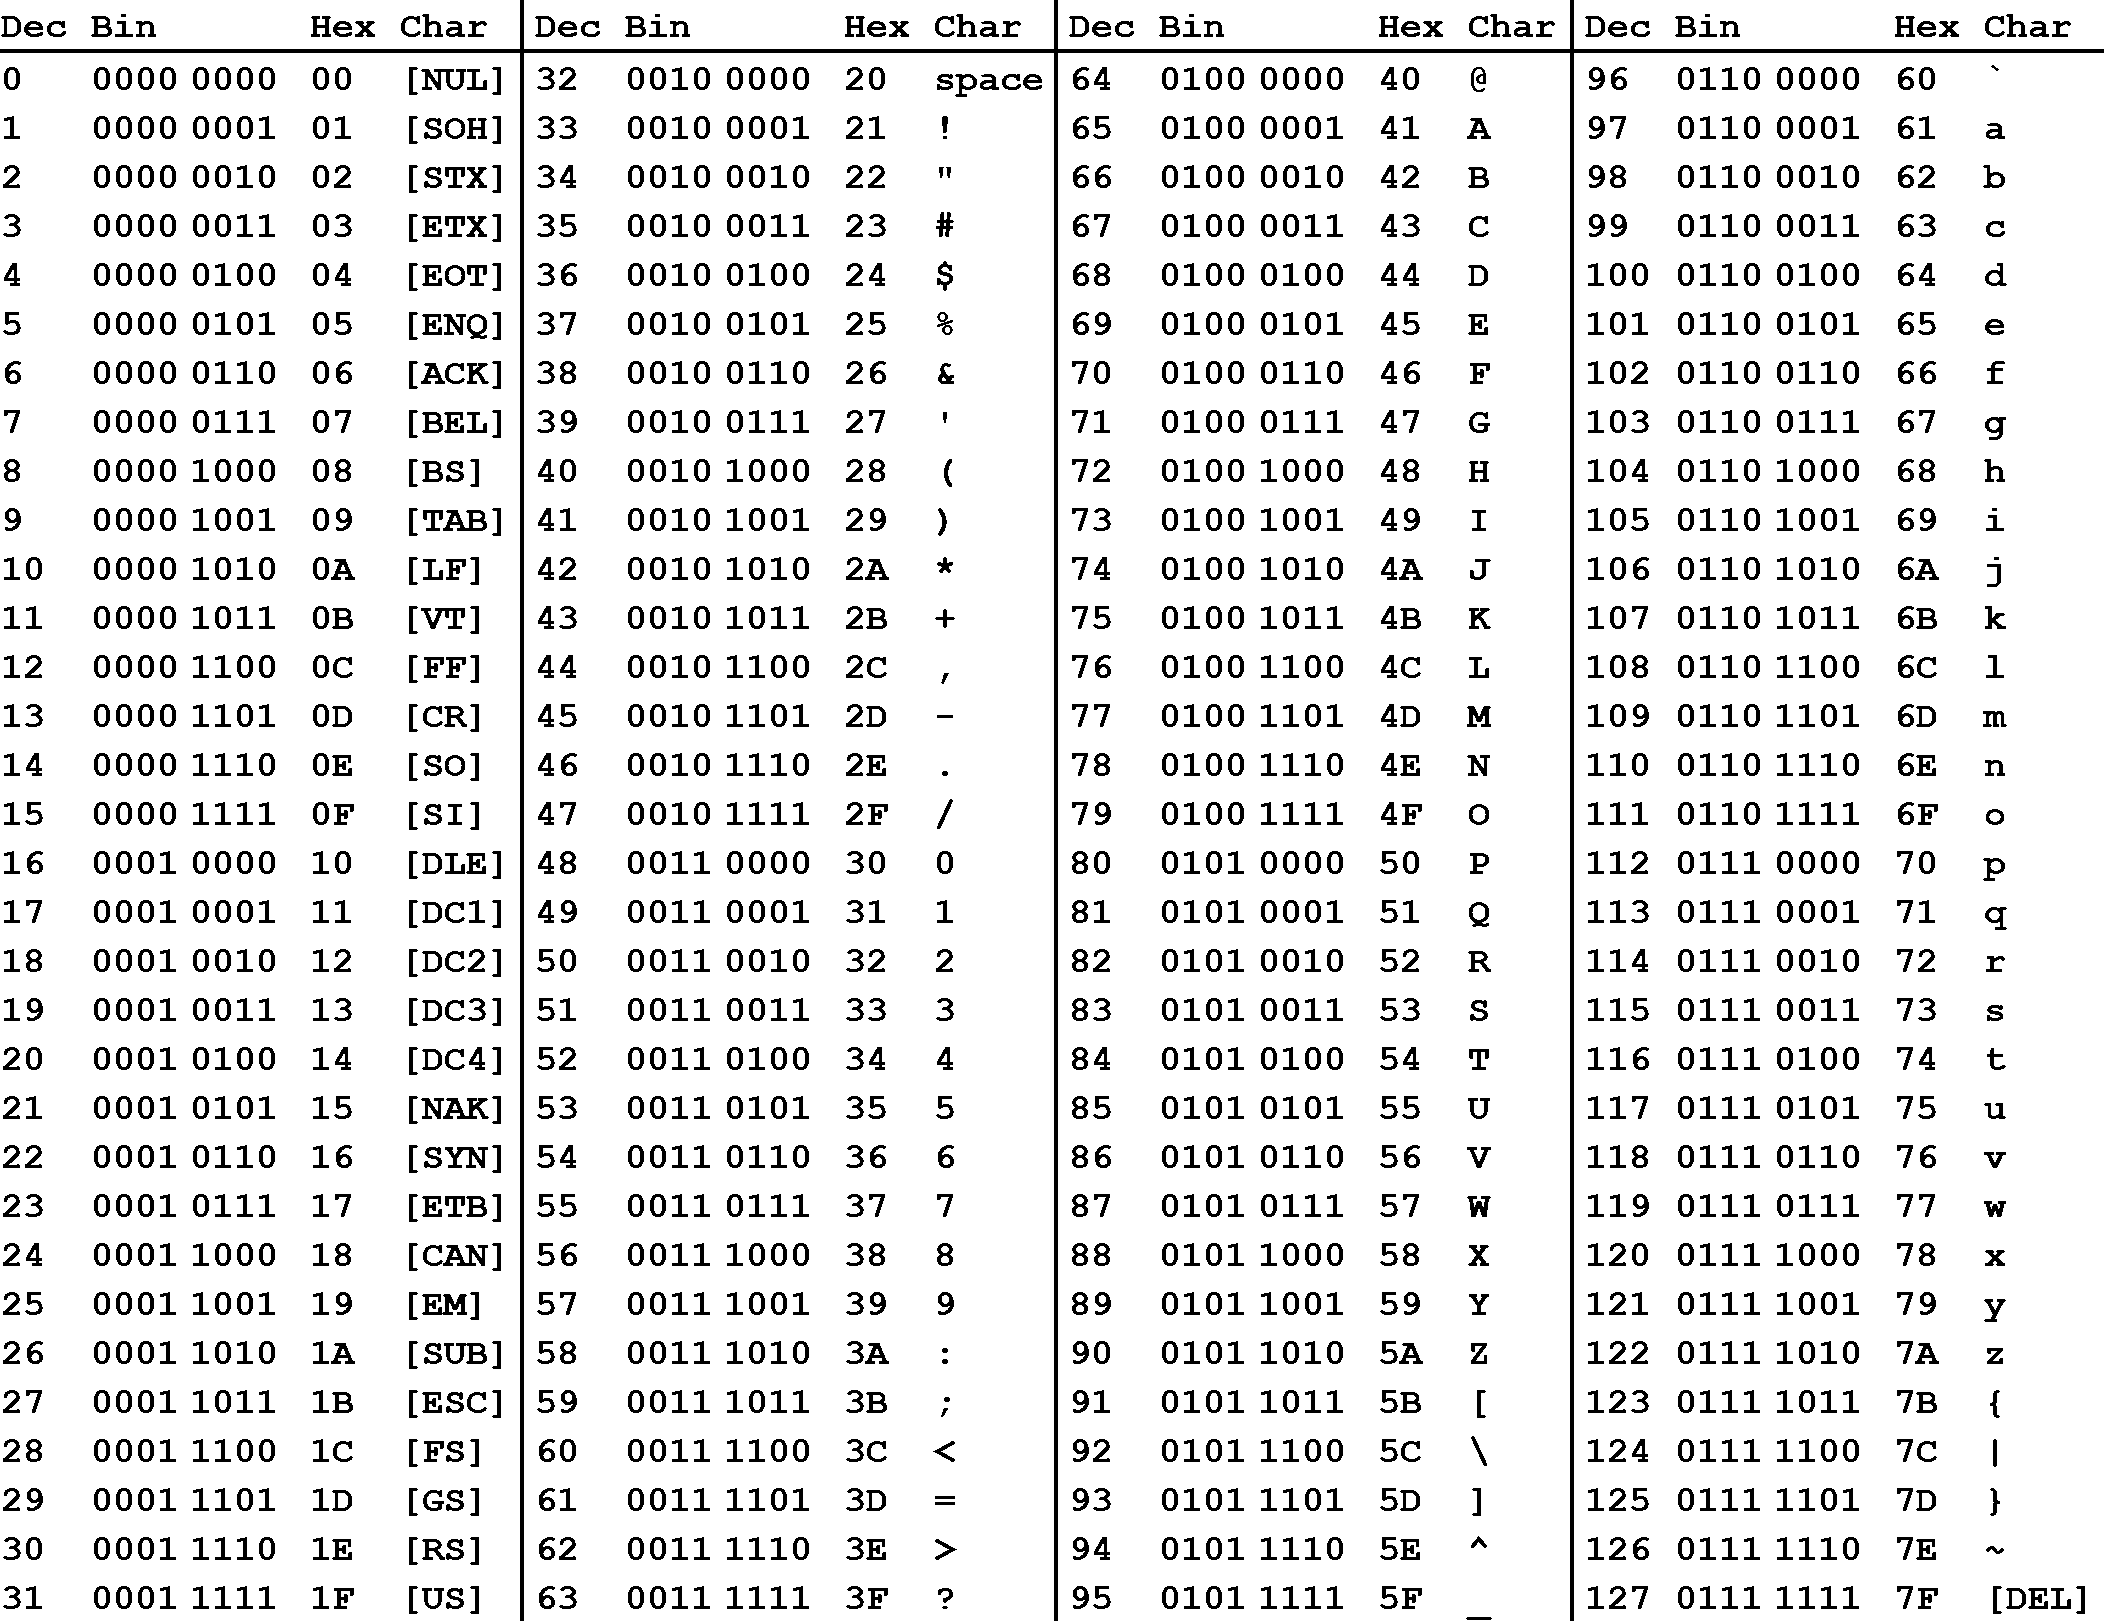
\includegraphics[width=\textwidth]{taticas/ascii.png}
\end{figure}

\newpage

\section{Tabela de Complexidades}
\begin{figure}[h]
	\centering
	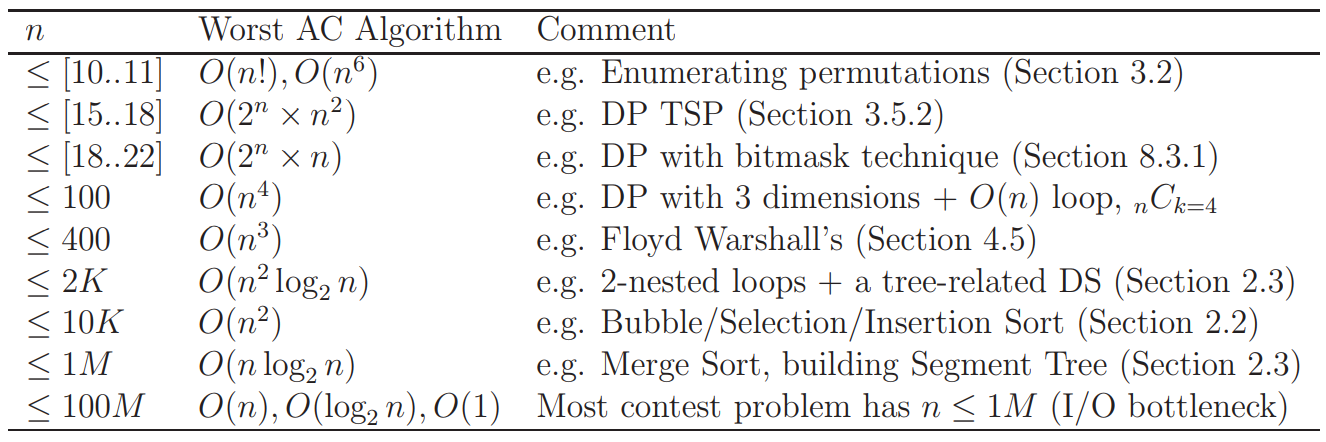
\includegraphics[width=\textwidth]{taticas/tab.png}
\end{figure}